\chapter{Literature Review}
\lhead{\leftmark}
\label{sec:review}
%
\section{Non-traditional Machining}
Non-traditional machining refers to a group of subtractive machining processes that remove the unwanted material from a workpiece using a number of techniques involving mechanical, thermal, electrical or chemical energy, or a combination of the aforementioned energies, but do not use a sharp cutting tool to remove material by plastic deformation or shearing.

\section{Electrodischarge Machining}
Electrodischarge Machining (EDM) is a non-traditional machining process where the removal of material is based on the electrodischarge erosion (EDE) effect of electric sparks occurring between two electrodes that are separated by a dielectric fluid. Metal removal occurs as a result of generation of extremely high heat generated by the high-energy sparks which melt and evaporate the two electrodes.
\subsection{The EDM Machining System}
The main components of the EDM system are shown in Fig. \ref{fig:edm}. These components include:
\begin{enumerate}
	\item The tool feed servo-controlled unit - This maintains a constant machining gap between the two electrodes, in order to ensure the occurrence of active discharges between them.
	\item Power supply - responsible for  supplying pulses at a certain voltage, current and duty cycle.
	\item Dielectric circulation unit - flushes the dielectric fluid to the inter-electrode gap after the machining debris has been filtered out. The dielectric fluid carries out a number of functions which are:
	\begin{itemize}
		\item Acts as a flushing medium and carries away the debris in the machining gap.
		\item Provides insulation between the electrode and the workpiece until the potential is sufficiently high.
		\item Cools down the sections heated by the electrodischarge effect.
	\end{itemize}
	\item Tool holder - holds the tool/wire being used to machine the workpiece.
	\item Filter - removes the machining debris from the dielectric fluid as it is being circulated in the system.
\end{enumerate}
\begin{figure}[h!]
	\centering
	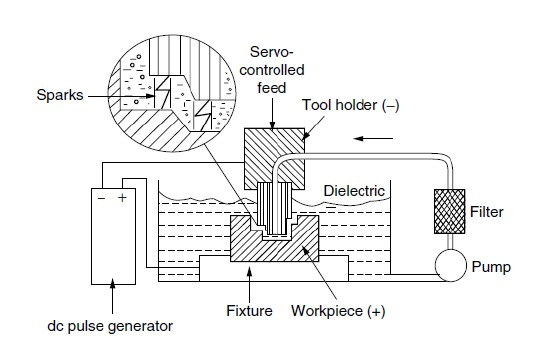
\includegraphics[width=0.7\linewidth]{Figures/edm}
	\caption{EDM Machining System Schematic}
	\label{fig:edm}
\end{figure}
\subsection{Wire EDM}
This is a special form of EDM, which uses a continuous wire which is constantly moving, called a wire electrode. It is used in the machining of superhard materials such as polycrystalline diamond(PCD) and Cubic Boron Nitride(CBN), and other matrix composites such as Tungsten carbide.

\subsection{EDM Process Parameters}
The EDM process can be used on any material that is an electrical conductor. The melting point and the latent heat of melting are important physical properties that determine the volume of metal removed per discharge.
%As these quantities increase, the rate of material removal decreases. The material-removal rate can be estimated from the approximate empirical formula:
%\newline
%\begin{align}
%	MRR = 4 \times 10^4 I\,T_w^-^1^.^2^3
%\end{align}
The performace of EDM is determined by a number of properties:
\begin{enumerate}
	\item Material Removal Rate (MRR)
	\item Surface Quality
	\item Accuracy
\end{enumerate}
These are determined by the process parameters such as:
\begin{itemize}
	\item Pulse characteristics
	\item Workpiece thermal properties - melting and boiling points, conductivity
	\item Dielectric properties
	\item Tool electrode - material, movement, wear
\end{itemize}

\subsection{Applications}
EDM has now become a vital process in modern manufacturing. It can manufacture intricate shapes with great precision from hard-to-machine materials like carbides, superalloys, and heat-resistant alloys. EDM can be incorporated within a computer-integrated manufacturing system to greatly cut down on the time a unit can operate without stopping for maintenance. Typically, EDM can be employed in:
\begin{enumerate}
	\item Micro-EDM: Micromachining of holes, slots and dies.
	\item EDM drilling - creation of cooling channels in turbines made of hard alloys.
	\item Electrodischarge sawing where billets and bars are created.
	\item Machining spheres, dies and moulds.
	\item EDM of ceramics used in insulation.
	\item Texturing - texturing is applied to the steel sheets during the final stages of cold rolling.
\end{enumerate}
\section{Other Non-Traditional Machining Processes}
\begin{enumerate}
\item Ultrasonic Machining - removal of hard and brittle materials using an axially oscillating tool at ultrasonic frequencies, with an abrasive slurry fed continuously into the machining zone between a soft tool and the workpiece.
\item Abrasive Jet Machining - using a focused stream of abrasive grains such as $Al_2O_3$ or $SiC$, carried by a high-pressure gas or air at a high velocity to impinge on the surface of a workpiece via a nozzle.
\item Chemical Machining - controlled chemical dissolution by contact with reagents or etchants, such as acids and alkaline solutions. Special coatings called maskants protect areas from which the material is not to be removed.
\item Electrochemical Machining - workpiece atoms are removed  by Electrochemical Dissolution (ECD) in accordance with Faraday's principles. Particles from the anodic material (workpiece), to the cathodic material (machining tool). It can be considered to be the opposite of electroplating.
\item Laser-beam Machining - the source of energy is a laser (an acronym for \textbf{L}ight \textbf{A}mplification by \textbf{S}timulated \textbf{E}mission of \textbf{R}adiation), which focuses optical energy on the surface of the workpiece. The highly focused, high-density energy source melts and evaporates portions of the workpiece in a controlled manner.
\item Abrasive Water Jet Machining - Water carried through a nozzle at high speed is used as the abrasive. A fine, high-pressure, high-velocity stream of water is directed at the work surface to cause cutting of the work.
\item Ice-Jet Machining - machining method that utilizes ice particles made from water instead of a mineral abrasive.
\end{enumerate}
\subsection{Design Considerations for EDM}
Some general design guidelines for EDM are as follows:
\begin{enumerate}
	\item Parts should be designed so that the required electrodes can be shaped properly and economically
	\item Deep slots and narrow openings should be avoided
	\item For economic production, the surface finish specified should not be too fine
	\item In order to achieve a high production rate, the bulk of material removal should be done by conventional processes (roughing out).
\end{enumerate}
% FDM uses aheating chamber to liquefy polymer that is fed into the system as a filament. The filament is pushed into the chamber by a tractor wheel arrangement and it is this pushing that generates the extrusion pressure. In this practical exercise, FDM was used to come up with a 3D object.
